\documentclass{article}
\usepackage[spanish]{babel}
\usepackage[utf8]{inputenc}
\usepackage[top=20mm, bottom=20mm, left=15mm, right=15mm]{geometry}
\usepackage{amsmath}
\usepackage{graphicx}
\usepackage{float}
\usepackage{listings}
\usepackage{color}
\usepackage[all]{xy}
\definecolor{codeblue}{RGB}{0,128,255}
\definecolor{codegray}{rgb}{0.5,0.5,0.5}
\definecolor{codepurple}{rgb}{0.58,0,0.82}
\definecolor{pink}{RGB}{255,26,117}
\definecolor{backcolour}{rgb}{1,1,1}
    
\lstdefinestyle{mystyle}{
    backgroundcolor=\color{backcolour},
    commentstyle=\color{codeblue},
    keywordstyle=\color{pink},
    numberstyle=\tiny\color{codeblue},
    stringstyle=\color{codepurple},
    basicstyle=\footnotesize,
    breakatwhitespace=false,         
    breaklines=true,                 
    captionpos=b,                    
    keepspaces=true,                 
    numbers=left,                    
    numbersep=7pt,                  
    showspaces=false,                
    showstringspaces=false,
    showtabs=false,                  
    tabsize=2,
    frame=tb
}

\lstset{style=mystyle}

\title{
    Reconocimiento de letras manuscritas con redes neuronales artificiales\\ 
    \large Tercera y cuarta entrega}
\author{Edson Raul Cepeda Marquez \\ Sonia Alejandra Treviño Rivera}
\date{\today}

\begin{document}
\setlength{\parskip}{2mm}
\setlength{\parindent}{0pt}
\maketitle
\section{Resumen}
Este proyecto consiste en una aplicación web que implementa una red neuronal artificial capaz 
de reconocer letras manuscritas. La aplicación web en cuestión está desarrollada con tres tecnologías 
que se conectan y permiten su uso:
\begin{enumerate}
    \item \textbf{Angular}: Un framework de código libre desarollado por Google que facilita el desarrollo de 
    aplicaciones web de una sola página (SPA: Single Page Applicaction). Tiene la ventaja de separar completamente el frontend y el backend lo que permite
    seguir facilmente el patrón de diseño MVC (Modelo-Vista-Controlador). 
    \item \textbf{Express}: Un framework de desarrollo web que utiliza el entorno de ejecución Node JS y facilita la creación de REST APIs.
    \item \textbf{Python}: Un lenguaje de programación interpretado orientado a objetos. Tiene la ventaja de ser simple, lo que permite escibir código legible.
    Tiene una amplia comunidad de desarrollo y una gran cantidad de librerias para todo tipo de tareas.
\end{enumerate}
En la figura \ref{flujo} se muestra un diagrama que representa el flujo de información entre las tres tecnologías. Se puede observar que la información fluye en ambas direcciones. 
\begin{figure}[H]
    \begin{displaymath}
        \xymatrix{*+<1cm>[F]{Angular} \ar[r] & *+<1cm>[F]{Express} \ar[l] \ar[r] & *+<1cm>[F]{Python} \ar[l]}
    \end{displaymath}
    \caption{Flujo de información de la aplicación.}
    \label{flujo} 
\end{figure}

La aplicación web además de contener este proyecto, tiene otras secciones asignadas para proyectos futuros. Para este proyecto la sección importante es ``Imchar''. 
Esta sección de la aplicación web contiene una cuadricula con la que se puede interactuar a traves del ratón. 
\begin{figure}[H]
    \centering
    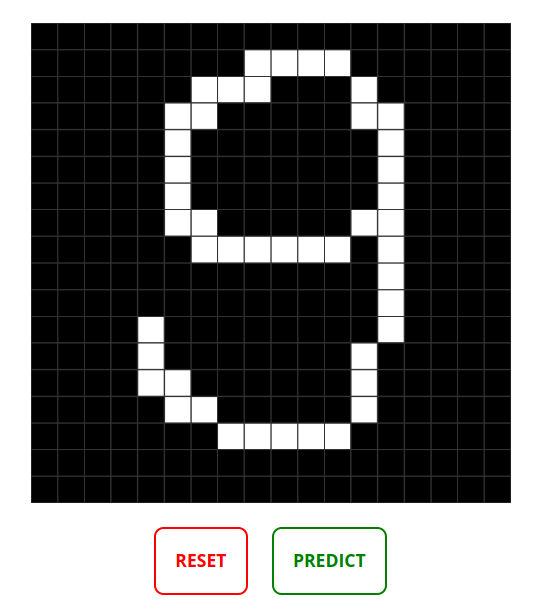
\includegraphics[width=40mm]{grid2.png}
    \caption{Cuadricula de la aplicación.}
    \label{grid}
\end{figure}
Esta es la puerta para el uso de la red neuronal artificial. 
En esta cuadricula es posible dibujar letras.
\\ Al dibujar una letra en la cuadricula y presionar el botón de ``Predeict'' la aplicación web realiza una petición al servidor de la REST API de express,
la cual recibe el estado de la cuadricula y sus dimensiones. \\
Posteriormente el servidor de express ejecuta un proceso asincrono de python el cual ejecuta un script que lleva a cabo una transformación de los datos enviados en la petición  \\
Por ultimo los datos transformados de la cuadricula son procesados por la red neuronal previamente entrenada, y devuelve una respuesta al frontend convertida en el caracter que la red neuronal predice (Figura \ref{response}).
\begin{figure}[H]
    \centering
    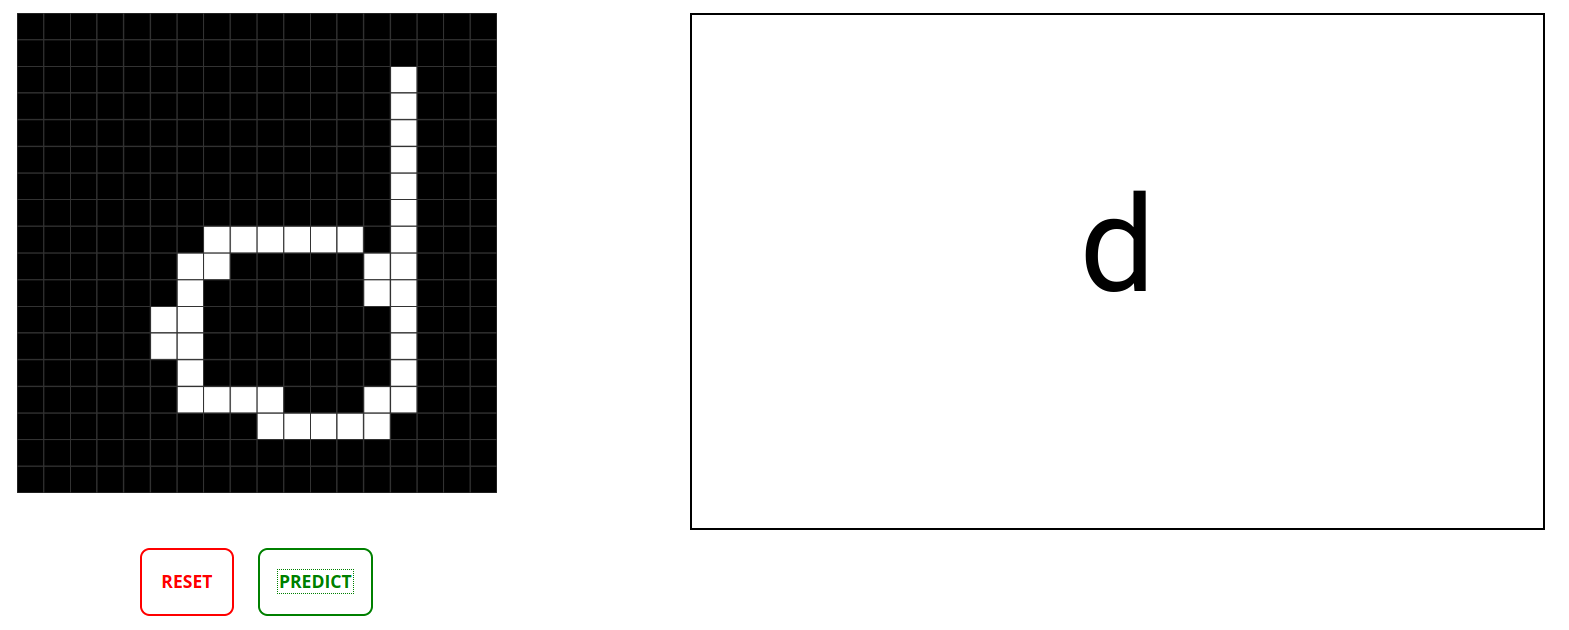
\includegraphics[width=180mm]{response.png}
    \caption{Respuesta de la red neuronal, también incluye el botón ``Reset'' para borrar la cuadricula.}
    \label{response}
\end{figure}
\textbf{Para el desarrollo de la red neuronal artificial no se utilizo ninguna librería, todo código correspondiente al algoritmo de aprendizaje fue escrito desde cero.} \\
Así mismo la red neuronal que procesa la información fue entrenada con un conjunto de datos creado desde cero, para esto se implemento una ruta oculta (figura \ref{trainer}) en la aplicación web en la que es posible utilizar la cuadricula para generar 
un conjunto de entranamiento.
\begin{figure}[H]
    \centering
    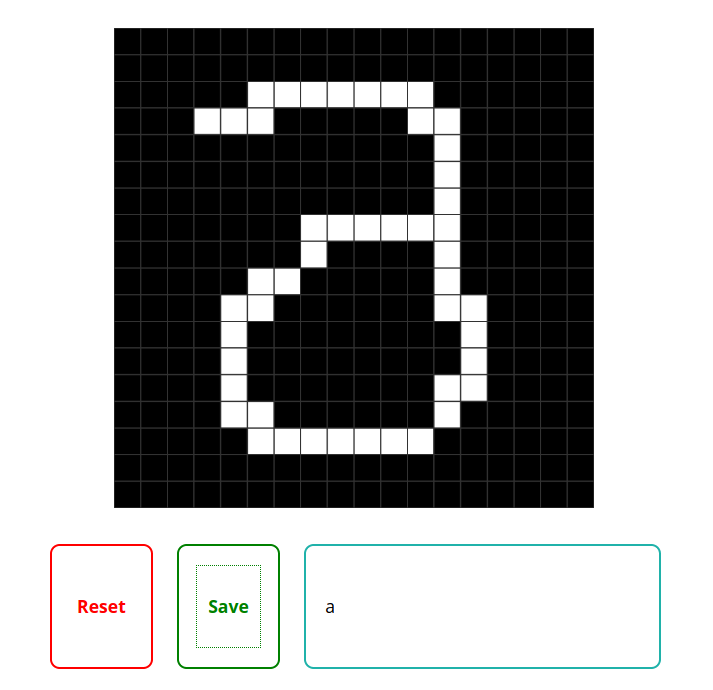
\includegraphics[width=60mm]{trainer.png}
    \caption{Ruta oculta para la generación de datos de entrenamiento}
    \label{trainer}
\end{figure}
Los resultados de entrenar la red neuronal con estos datos son que, para las 26 letras del abecedario en ingles por lo menos 21 son predichas correctamente. Las letras que presentan más problemas para ser predichas correctamente son aquellas que 
comparten cierta similaridad. La red neuronal fue entrenada multiples veces para poder llegar a una configuración de hiperparametros con un mejor rendimiento. 

\section{Introducción}
El problema que se intenta resolver al diseñar este sistema, es el de reconocer texto manuscrito para su digitalización. 
Se diseña una red neuronal convolucional que es entrenada 
\end{document}El flujo de información entre las tres herramientas 
